\documentclass[
%% TIKZ_CLASSOPTION %%
tikz
]{standalone}
\usepackage{amsmath}
\usetikzlibrary{matrix}
%% EXTRA_TIKZ_PREAMBLE_CODE %%
\begin{document}
%% TIKZ_CODE %%

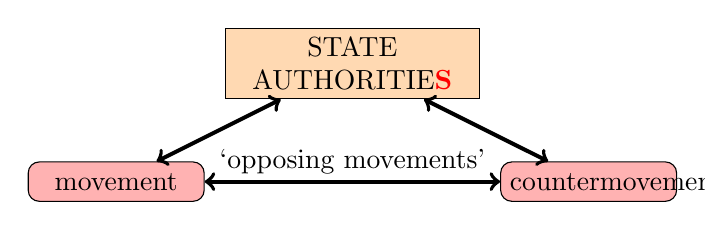
\begin{tikzpicture}[node distance=3cm]

\tikzstyle{BOX} = [rectangle, rounded corners, minimum width=2cm, minimum height=0.5cm,text centered, text width=2cm, draw=black, fill=red!30]
\tikzstyle{RECT} = [rectangle, minimum width=1cm, minimum height=0.5cm, text centered, text width=3cm, draw=black, fill=orange!30]
\tikzstyle{arrow} = [thick,->,>=stealth]

\node (STATE) [RECT] {STATE \linebreak AUTHORITIE\textcolor{red}{\textbf{S}}};
\node (move) [BOX, below of=STATE, xshift=-3cm, yshift=1.5cm] {movement};
\node (cmove) [BOX, below of=STATE, xshift=3cm, yshift=1.5cm] {countermovement};
\node [below of=STATE, yshift=1.75cm] {`opposing movements'};

\draw[line width=0.5mm, <->] (STATE) to (move);
\draw[line width=0.5mm, <->] (STATE) to (cmove);
\draw[line width=0.5mm, <->] (move) to (cmove);

\end{tikzpicture}

\end{document}
